\chapter{Experiments}\label{chapter:experiments_and_results}
As mentioned in the previous chapter, the process of finding was an iterative one of running an experiment, analyzing the generated data, draw conclusions and then repeat the steps with a new experiments designed to amend the mistakes of the previous experiment. This chapter will go through each of these steps and explain the insights that were gained.

This chapter presents the flow of analysis as it was carried out, rather 

A summary and discussion of the results is found in chapter \ref{chapter:discussion}.


\section{D3}
In this experiment, the number of \ssmmnAgents and \scnAgents as well all the latency parameters were included in the individuals. The genetic algorithm was run for 1000 generations with a population size of 200. A total of 


This data set was generated by including all the model parameters concerning time latency as well as the number of agents into the individuals in the genetic algorithm. Due to the high number of variables, the data turned out to be difficult to analyze, as too many factors pertaining to the simultaneous change of several parameters influenced the fitness values. Thus, not many definitive results concerning the impact of time latency of market behavior were derived from this data set. The reason why it is still included in the thesis is that the data did provide hints on how to proceed with the analysis of the model. Furthermore, the data set proved useful for developing the tools used to analyze the data sets that were generated later, and hence this section is intended to illustrate the motivation for applying these tools.

Scatter plots of the fitness data before and after preprocessing were already shown in figure \ref{figure:scatter_log_transform}.

\begin{table}
	\centering
	\begin{tabular}{l|l}
	Dataset id & Parameters in genes\\
	\dthree & \sclatencymu, \sclatencys, \scnAgents, \scthinkmu, \scthinks, \sctimehorizonmu, \sctimehorizons, \scwaitTimeBetweenTradingmu, \scwaitTimeBetweenTradings, \ssmmlatencymu, \ssmmlatencys, \ssmmnAgents, \ssmmthinkmu, \ssmmthinks	
	\end{tabular}
\end{table}

Free parameters:

Data set \dthree was the first run of the genetic algorithm that actually produced something that looked like results. The following parameters were included in the genetic algorithm individuals:
\begin{center}
\sclatencymu, \sclatencys, \scnAgents, \scthinkmu, \scthinks, \sctimehorizonmu, \sctimehorizons, \scwaitTimeBetweenTradingmu, \scwaitTimeBetweenTradings, \ssmmlatencymu, \ssmmlatencys, \ssmmnAgents, \ssmmthinkmu, \ssmmthinks
\end{center}

Fixed parameters:




\begin{figure}
	%issue 15
	\centering
	\subcaptionbox{Evolution of \ssmmlatencymu and \sclatencymu}
	[0.49\linewidth]{\includegraphics[width=0.5\textwidth]{82_generation_plots/d3/latpars_mu.png}}
	\subcaptionbox{Evolution of \ssmmthinkmu and \scthinkmu}
	[0.49\linewidth]{\includegraphics[width=0.5\textwidth]{82_generation_plots/d3/thinkpars_mu.png}}
	\subcaptionbox{Evolution of \ssmmnAgents and \scnAgents}
	[0.49\linewidth]{\includegraphics[width=0.5\textwidth]{82_generation_plots/d3/nAgents.png}}
	\caption{Evolution of time delay parameters common both HFT agent types, and of the number of agents in experiment \dthree}\label{fig:d3_evolution_latpars_nAgents}
\end{figure}


\begin{figure}
	%issue 15
	\subcaptionbox{Evolution of \sctimehorizonmu}
	[0.49\linewidth]{\includegraphics[width=0.5\textwidth]{82_generation_plots/d3/sctimehorizon_mu.png}}
	\subcaptionbox{Evolution of \scwaitTimeBetweenTradingmu}
	[0.49\linewidth]{\includegraphics[width=0.5\textwidth]{82_generation_plots/d3/scwaittime_mu.png}}
	\caption{Evolution of chartist-specific strategy parameters in experiment \dthree}\label{fig:d3_evolution_thinkpars}
\end{figure}

\begin{figure}
	%issue 15
	\centering
	\subcaptionbox{Evolution of \roundstable}
	[0.49\linewidth]{\includegraphics[width=0.5\textwidth]{82_generation_plots/d3/round_stable.png}}
	\subcaptionbox{Evolution of \timetoreachnewfundamental}
	[0.49\linewidth]{\includegraphics[width=0.5\textwidth]{82_generation_plots/d3/time_to_reach_new_fundamental.png}}
	\subcaptionbox{Evolution of \stdev}
	[0.49\linewidth]{\includegraphics[width=0.5\textwidth]{82_generation_plots/d3/stdev.png}}
	\subcaptionbox{Evolution of \overshoot}
	[0.49\linewidth]{\includegraphics[width=0.5\textwidth]{82_generation_plots/d3/overshoot.png}}
	\caption{Evolution of the four fitness measures in experiment \dthree}\label{fig:d3_evolution_fitness}
\end{figure}


EVEN THOUGH ROUND STABLE AND TIME TO REACH NEW FUNDAMENTAL SEEM SIMILAR, THEY ARE NOT CORRELATED SO MUCH. WRITE ABOUT WHAT THIS MEANS (e.g. some markets reach new fundamental quickly, but never become stable, etc.)

\subsection{Section summary}
In summary, the main problem with this data set was that it contained mostly simulations with few or no high frequency traders. 

\section{D9: Fixing the number of high frequency traders}

\subsection{Parameter and fitness evolution}

\begin{figure}
	%issue 15
	\centering
	\subcaptionbox{Evolution of \ssmmlatencymu and \sclatencymu}
	[0.49\linewidth]{\includegraphics[width=0.5\textwidth]{82_generation_plots/d9/latpars_mu.png}}
	\subcaptionbox{Evolution of \ssmmthinkmu and \scthinkmu}
	[0.49\linewidth]{\includegraphics[width=0.5\textwidth]{82_generation_plots/d9/thinkpars_mu.png}}
	\caption{Evolution of time delay parameters common both HFT agent types in experiment \dthree}
	\label{fig:d9_evolution_latpars}
\end{figure}


\begin{figure}
	%issue 15
	\subcaptionbox{Evolution of \sctimehorizonmu}
	[0.49\linewidth]{\includegraphics[width=0.5\textwidth]{82_generation_plots/d9/sctimehorizon_mu.png}}
	\subcaptionbox{Evolution of \scwaitTimeBetweenTradingmu}
	[0.49\linewidth]{\includegraphics[width=0.5\textwidth]{82_generation_plots/d9/scwaittime_mu.png}}
	\caption{Evolution of chartist-specific strategy parameters in experiment \dnine}
	\label{fig:d9_evolution_thinkpars}
\end{figure}



\begin{figure}
	%issue 15
	\centering
	\subcaptionbox{Evolution of \roundstable}
	[0.49\linewidth]{\includegraphics[width=0.5\textwidth]{82_generation_plots/d9/round_stable.png}}
	\subcaptionbox{Evolution of \timetoreachnewfundamental}
	[0.49\linewidth]{\includegraphics[width=0.5\textwidth]{82_generation_plots/d9/time_to_reach_new_fundamental.png}}
	\subcaptionbox{Evolution of \stdev}
	[0.49\linewidth]{\includegraphics[width=0.5\textwidth]{82_generation_plots/d9/stdev.png}}
	\subcaptionbox{Evolution of \overshoot}
	[0.49\linewidth]{\includegraphics[width=0.5\textwidth]{82_generation_plots/d9/overshoot.png}}
	\caption{Evolution of the four fitness measures in experiment \dnine}
	\label{fig:d9_evolution_fitness}
\end{figure}

\subsection{Visualizing the data set}
\begin{figure}
\centering
\subcaptionbox{$\log \stdev$ vs. $\log \roundstable$ vs. \timetoreachnewfundamental}
[0.49\linewidth]{\includegraphics[width=0.5\textwidth]{21_scatter_plots/d9/d.png}}
\subcaptionbox{\roundstable vs. \timetoreachnewfundamental vs. \stdev}
[0.49\linewidth]{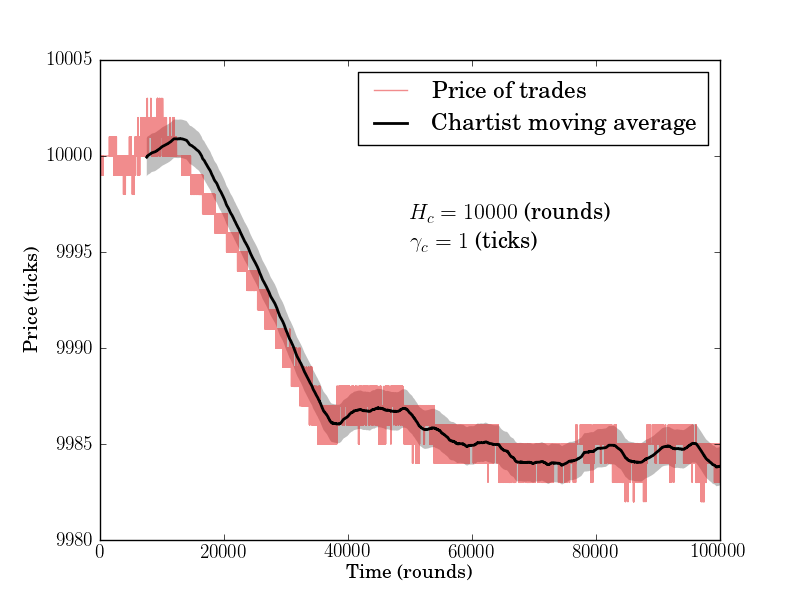
\includegraphics[width=0.5\textwidth]{21_scatter_plots/d9/c.png}}
\subcaptionbox{$\log \overshoot$ vs . $\log \stdev$ vs. \timetoreachnewfundamental}
[0.49\linewidth]{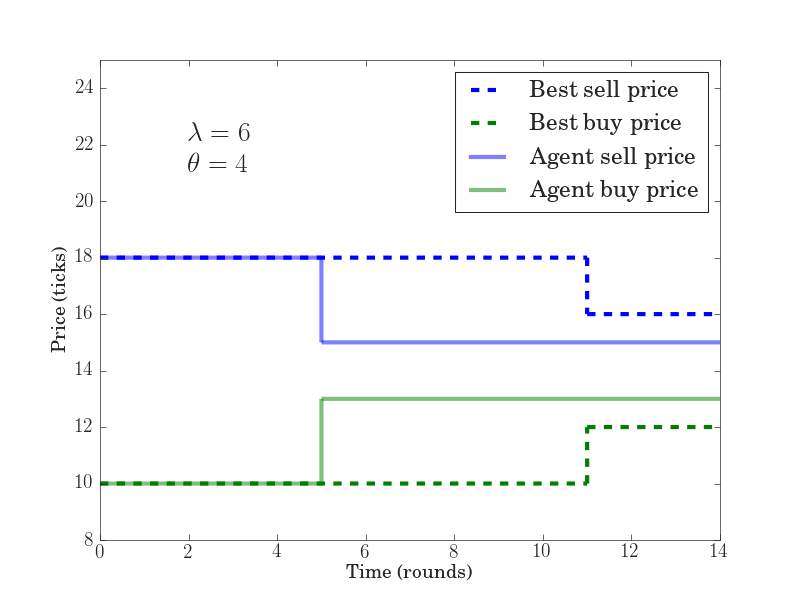
\includegraphics[width=0.5\textwidth]{21_scatter_plots/d9/b.png}}
\caption{Scatter plots of fitness measures in experiment \dnine. }
\label{figure:d9_scatter_fitness}
\end{figure}



\begin{enumerate}
\item It rarely happens that a market has a large overshoot, and then returns to a stable state (large \overshoot, small \stdev)
\item 
\end{enumerate}


The scatter plots do seem to reveal some structure, the presence of large values in the \stdev feature obscures the nature of this structure, in spite of the logarithmic scaling. The plot showing $\log \stdev$ vs. $\log \roundstable$ is squeezed to the left, and the color grading on the scatter plot for $\log \overshoot$ vs . $\log \stdev$ reveals no variety in the \stdev feature. In an attempt to get some more information out of the scatter plot, data points with a more than 100 \% overshoot (corresponding to $\overshoot > 10$ ) are removed. The resulting scatter plots for the reduced data set are shown and discussed in the section \ref{section:d9_analysing_scatter_plots}.

\subsection{Analysing scatter plots}\label{section:d9_analysing_scatter_plots}

\subsubsection{\roundstable vs \stdev}
\begin{figure}
\centering
\includegraphics[width=0.7\textwidth]{103_scatter_manual_outlier/d9/d.png}
\caption{Scatter plot of $\log \stdev$, $\log \roundstable$ and \timetoreachnewfundamental}
\label{figure:d9_scatter_fitness_inliers_logs_logr_t}
\end{figure}

\begin{figure}
\centering
\includegraphics[width=0.7\textwidth]{103_scatter_manual_outlier/d9/l.png}
\caption{Scatter plot of $\log \stdev$, $\log \roundstable$ and \overshoot}
\label{figure:d9_scatter_fitness_inliers_logs_logr_o}
\end{figure}



\subsubsection{\roundstable vs. \timetoreachnewfundamental}
\begin{figure}
\centering
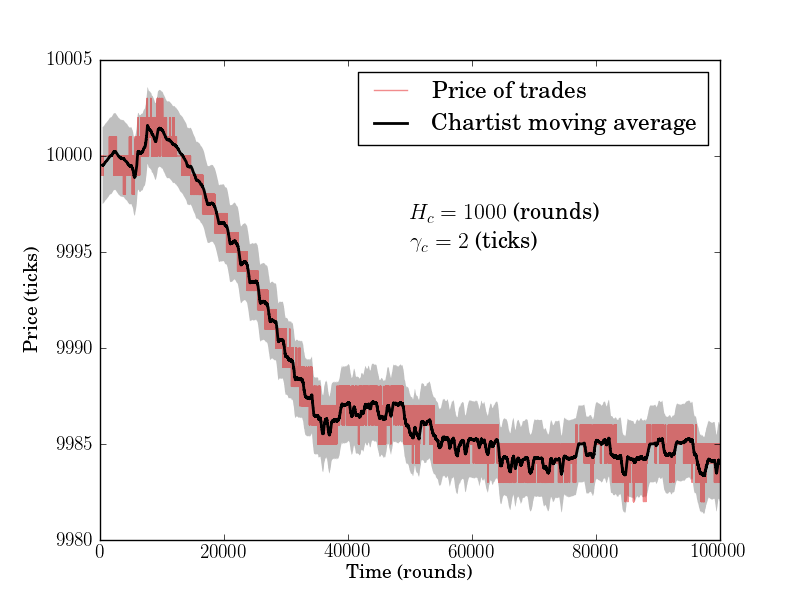
\includegraphics[width=0.7\textwidth]{103_scatter_manual_outlier/d9/f.png}
\caption{Scatter plot of \roundstable, \timetoreachnewfundamental and \stdev}
\label{figure:d9_scatter_fitness_inliers_t_r_logs}
\end{figure}
\begin{figure}
\centering
\includegraphics[width=0.7\textwidth]{103_scatter_manual_outlier/d9/j.png}
\caption{Scatter plot of \overshoot, $\log \roundstable$ and \timetoreachnewfundamental}
\label{figure:d9_scatter_fitness_inliers_t_r_o}
\end{figure}

The line $\timetoreachnewfundamental = \roundstable$ (black dashed line) divides figure \ref{figure:d9_scatter_fitness_inliers_t_r_logs} into region A, (upper left triangle) and region B (lower right triangle). Region A contains the fitness-points of the simulations which are counted as stable \textit{after} they reach the new fundamental, and region B contain those that become stable before. Comparing with 



\begin{enumerate}
\item In figure \ref{figure:d9_scatter_fitness_inliers_t_r_logs}, the density of points is slightly higher around the region defined by $\roundstable = \timetoreachnewfundamental$. This is true both for small and large values of \timetoreachnewfundamental and \roundstable. Furthermore, these points all have small values for $\stdev$. The same points can be identified by looking at figure \ref{figure:d9_scatter_fitness_inliers_a}, where a cloud of points lay around the vertical line $\log \stdev \approx -0.6$.
\begin{enumerate}
	\item The low \stdev means that the traded price is stable after entering the stability margin. Furthermore, the simulations represented by these same points are among the ones with the most stable traded prices.
	%\item Because of the high correlation between \stdev and \overshoot, simulations belonging to this group have little or no overshoot. 
	\item Since $\timetoreachnewfundamental \approx \roundstable$, the traded does not leave the stability margin once it has entered. This is true for both small and large values of \timetoreachnewfundamental and \roundstable.
\end{enumerate}
\item In figure \ref{figure:d9_scatter_fitness_inliers_t_r_logs} The density seems high in the region defined by the inequalities $0.2 < \timetoreachnewfundamental < 0.3$ and $\roundstable > 0.25$. 
	\begin{enumerate}
	\item Simulations in this group reach the new fundamental quickly (less than $2\cdot 10^4$ rounds after the shock), but then leave the stable region again.
	\item The simulations which take a longer time to become stable also have less stable traded prices (higher values of \stdev)
	\end{enumerate}
\end{enumerate}



\subsubsection{\stdev vs. \timetoreachnewfundamental}
\begin{figure}
\centering
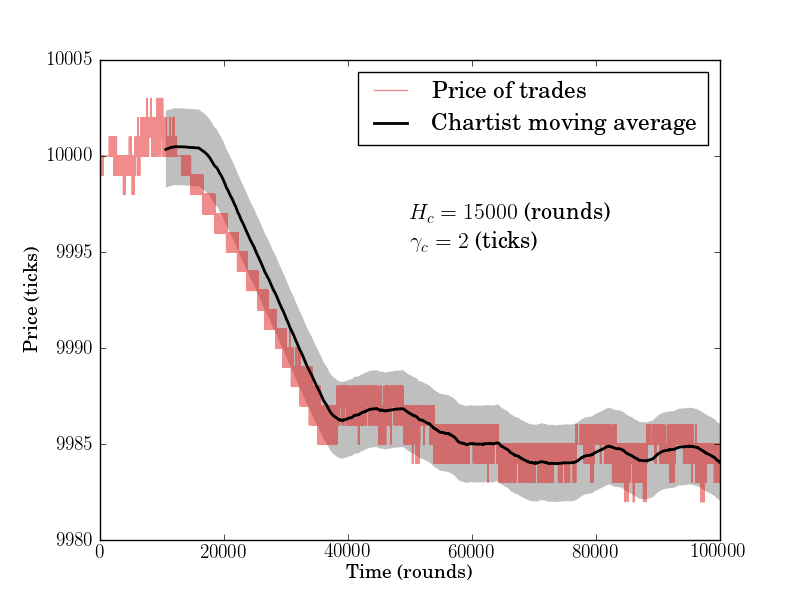
\includegraphics[width=0.7\textwidth]{103_scatter_manual_outlier/d9/h.png}
\caption{Scatter plot of \roundstable, \timetoreachnewfundamental and \stdev}
\label{figure:d9_scatter_fitness_inliers_logs_t_r}
\end{figure}
\begin{figure}
\centering
\includegraphics[width=0.7\textwidth]{103_scatter_manual_outlier/d9/k.png}
\caption{Scatter plot of \roundstable, \timetoreachnewfundamental and \overshoot}
\label{figure:d9_scatter_fitness_inliers_logs_t_o}
\end{figure}

\begin{enumerate}
\item The two large clusters of red points in figure \ref{figure:d9_scatter_fitness_inliers_c} are all the simulations which never became stable during the simulation. The horizontal cluster contain the simulations which responded quickly to the shock by taking only between 10.000 and 20.000 rounds. This cluster contains simulations with both high and low \stdev values, indicating varied behavior.
\item The spike of points on the right side of the cluster are simulations that did become stable, but did so slowly and with no overshoot, as is seen by observing that all the points in the cluster are blue when the color indicated the value of \overshoot as in figure \ref{figure:d9_scatter_fitness_inliers_logs_t_o}.
\end{enumerate}











The next section seeks an answer to the question of whether or not there are model parameters which cause the model to behave in certain ways.
In other words, is it possible to make predictions about the model behavior based of the model parameters?










\subsection{Looking for parameters causing certain behavior}
In order to answer the question posed in the end of the previous section, we can divide the data points into groups based on their fitness values, and then calculate descriptive statistics for the parameters of the points belonging to each group. 

The easiest first step is to do that for the outliers and inliers.


\begin{figure}
\subcaptionbox{}
[0.49\linewidth]{\includegraphics[width=0.5\textwidth]{101_pars_vs_fits/d9/ssmm_latency_mu__vs__round_stable(mean)_scatter.png}}
\subcaptionbox{}
[0.49\linewidth]{\includegraphics[width=0.5\textwidth]{101_pars_vs_fits/d9/ssmm_latency_mu__vs__round_stable(median)_scatter.png}}
\caption{}
\label{figure:d9_parvsfit_ssmm_latency_mu__vs__round_stable(median)_scatter}
\end{figure}




As manually labeling hundreds of thousands of data points is not really an option, clustering algorithms were used to separate the fitness data into groups with distinct characteristics. 

\subsection{Section summary}


\section{D10}
In the previous section, some weak tendencies 
The scatter plots for \dten{} are somewhat similar to those of \dnine, and they have therefore been placed in appendix \ref{appendix:figures}





Note that the definition of ``nice'' market behavior is, of course, qualitative in nature. In this experiment, as well as in \dnine{} and \deleven, the search for such nice behavior was carried out by minimizing all four fitness measures, as nice market behavior was taken to be a market that . Whether this can be accomplished by the model or not is a question that can only be answered by running the 

If, say, a fast reaction on the cost of a larger overshoot, one could search for such behavior by omitting \overshoot{} from the optimization criteria.



Figure \ref{fig:d10_evolution_fitness} shows the evolution of the four fitness measures. The population wide mean is plotted along the median and minimum statistics. Since all four fitness measures were minimized, the curve for the minimum value shows the best individual alive during each generation, with respect to each fitness measure. While the mean reflects how the overall population is evolving,  the median is useful as it gives an insight into how skewed the population wide distribution of parameters is. 
\begin{figure}
	%issue 15
	\centering
	\subcaptionbox{Evolution of \roundstable\label{fig:d10_evolution_fitness_a}}
	[0.49\linewidth]{\includegraphics[width=0.5\textwidth]{82_generation_plots/d10/round_stable.png}}
	\subcaptionbox{Evolution of \timetoreachnewfundamental\label{fig:d10_evolution_fitness_b}}
	[0.49\linewidth]{\includegraphics[width=0.5\textwidth]{82_generation_plots/d10/time_to_reach_new_fundamental.png}}
	\subcaptionbox{Evolution of \stdev\label{fig:d10_evolution_fitness_c}}
	[0.49\linewidth]{\includegraphics[width=0.5\textwidth]{82_generation_plots/d10/stdev.png}}
	\subcaptionbox{Evolution of \overshoot\label{fig:d10_evolution_fitness_d}}
	[0.49\linewidth]{\includegraphics[width=0.5\textwidth]{82_generation_plots/d10/overshoot.png}}
	\caption{Evolution of the four fitness measures in experiment \dten}
	\label{fig:d10_evolution_fitness}
\end{figure}



\subsection{Fitness and parameter evolution}\label{section:fitness_and_paraeter_evolution}
Figure \ref{fig:d10_evolution_fitness} show the evolution of the population wide mean, median and minimum statistics for each of the four fitness-measures. 
\begin{description}
\item[Model stability]
Figure \ref{fig:d10_evolution_fitness_a}: shows that  the GA quickly manages to find some parameters which cause the simulation to stabilize quickly. However, these individuals do not manage to dominate the population evident by the mean and median curves remaining almost the same until generation 30 or so. In the next 20 generations the population undergoes a rapid change, as the population wide average of \roundstable drop from close to $10^5$ to around $2\cdot 10^4$ rounds on average. The disparity between the mean and the median indicates that the population undergoes a rapid change in the same period, from mostly containing unstable individuals to mostly containing stable individuals. In generation 42, the median curve crosses the mean curve, which means that the the population contain as many stable simulations as it contain unstable simulations. From that point on the unstable simulations are quickly replaced by stable individuals.
\item[Price fluctuations and overshoot] During the same period, the population average \stdev also decreases fairly rapidly, but the drop is less pronounced than the drop in \stdev. As figures \ref{fig:d10_evolution_parameters_a} and \ref{fig:d10_evolution_parameters_b} show, the number of market makers rapidly increased during this period, as did the average latency of the market makers. Since the mean and median are close in both figure\footnote{Since \overshoot is discrete, the median and $\min$ statistics are also discrete}, the mean is representative of the evolution of the entire population.
\item[Responsiveness] \timetoreachnewfundamental measures the time it takes for the model to react to the shock in the fundamental, and the evolution of the population wide statistics is shown on figure \ref{fig:d10_evolution_fitness_b}. Although the GA is instructed to minimize \timetoreachnewfundamental in order to look for more faster models, it clearly fails to do this. Indeed, the most responsive simulation took only about 4000 rounds to reach the new fundamental, but this individual died out in favor of slower individuals. In the last generation the most responsive simulation took around 14000 rounds to reach the new fundamental. The reasons for this failure to locate responsive models is discussed in section \ref{section:correlation_fitness}. In the A large change of the average of \timetoreachnewfundamental happens in the rounds five to 15. In this period, the median is lower than the mean, which means that the growth in the mean can be attributed to a minority of individuals.
\end{description}

On figures \ref{fig:d10_evolution_fitness} and \ref{fig:d10_evolution_parameters}, the two areas shaded in a light blue and light red respectively show the two periods during which there was a drastic change in parameters and fitness-values. By comparing the time at which parameters and fitness-values change, it is possible to get an idea of how parameters influence the fitness-values. To that end, figure \ref{fig:d10_evolution_parameters} shows the evolution of each of the parameters that were varied by the GA\footnote{Since the median was found to follow the mean nicely for all the parameters, the medians are not displayed. Also, the gray error bars show the population wide variance}.
\begin{figure}
	%issue 15
	\centering
	\subcaptionbox{Evolution of \ssmmlatencymu{} and \sclatencymu\label{fig:d10_evolution_parameters_a}}
	[0.49\linewidth]{\includegraphics[width=0.5\textwidth]{82_generation_plots/d10/latpars_mu.png}}
	\subcaptionbox{Evolution of \ssmmlatencys{} and \sclatencys\label{fig:d10_evolution_parameters_b}}
	[0.49\linewidth]{\includegraphics[width=0.5\textwidth]{82_generation_plots/d10/latpars_s.png}}
	\subcaptionbox{Evolution of \ssmmnAgents\label{fig:d10_evolution_parameters_c}}
	[0.49\linewidth]{\includegraphics[width=0.5\textwidth]{82_generation_plots/d10/nAgents.png}}
	\caption{Evolution of the model parameters in experiment \dten}
	\label{fig:d10_evolution_parameters}
\end{figure}

The two periods indicated by the shaded squares seem to reflect some sudden changes in the parameters.

\begin{description}
\item[Average agent latency]  As is shown on figure \ref{fig:d10_evolution_parameters_a}, individuals containing large latency parameters are selected for both HFT market makers and HFT chartists. $\E{\sclatencymu}$ grows grows quickly during the first 20 rounds (blue shade). Referring back to figure \ref{fig:d10_evolution_fitness}, it is seen that $\E{\timetoreachnewfundamental}$ and $\E{\overshoot}$ grows and shrinks respectively. As for $\E{\ssmmlatencymu}$, it grows from rounds 20 through 50 (red shade), and this  seems to be strongly reflected in the growth of $\E{\roundstable}$, and to a lesser degree a decline in $\E{\overshoot}$ and $\E{\stdev}$. Furthermore, the small size of the error bars on both curves show that the population consistently moves towards containing more individuals with larger latency parameters for both HFT agent types. While initially $\E{\ssmmlatencymu} \approx \E{\sclatencymu}$, the population wide mean $\E{\sclatencymu}$ ends up being roughly 1.5 times larger than $\E{\sclatencymu}$. Finally, note also that the growth of  $\E{\sclatencymu}$ and $\E{\ssmmlatencymu}$ seem to be somewhat independent, as they sometimes grow together, sometimes not.

\item[Number of market makers] The number of market makers increases almost every generation, but grows especially quickly through rounds 20 to 50 (red shade)

\item[Agent latency variance] Figure \ref{fig:d10_evolution_parameters_b}: The trends for $\E{\sclatencys}$ and $\E{\ssmmlatencys}$ are less clear, as the population-wide variances $\Var{\sclatencymu}$ and $\ssmmlatencymu$ illustrated by the large error bars are high compared to the change in $\E{\sclatencymu}$ and $\E{\ssmmlatencymu}$. While this could mean that the simulation behaves more nicely when the difference between the latency parameters of the trading agents is smaller, further experiments would have to be carried out to confirm this fact. XXX
\end{description}

In summary, the genetic algorithm prefers simulations with many, but relatively slow market makers. Apparently simulations with slow chartists also outperformed those with fast chartists, but since the number of HFT chartists was fixed at $\scnAgents = $, this experiment does not reveal how the simulation would perform with more (or less) chartists. It is possible to imagine that the market would perform just as well with a few and fast chartists. Section \ref{section:experiment_11} contains the analysis of an experiment in which the number of chartists were varied. The discussion above can be summarized as follows:

\begin{enumerate}
\item The responsiveness of the market is influenced by latency of the chartists. Slower chartists made the market require more time to respond to the fundamental shock.
\item The time it takes for the market to become in influenced by the number of market makers and on the latency of the market makers. More but slower market makers seems to make the market settle within the stability margin faster.
\item The overshoot, as well as the average size of the price fluctuations of the market, are both influenced by the latency of both agent types, as well as the number of market makers.
\item The market was more stable but reacted slowly when the chartists were slower than the market makers.
\end{enumerate}
The accuracy of the above analysis is limited as it only looks at population wide statistics at a given point in the duration of the GA. The following section contain an analysis in which the generation to which each data point belongs is considered irrelevant. The analysis will try to confirm each of the four statements above.




\subsection{Correlation between fitness measures}\label{section:correlation_fitness}
A factor which influences the evolution of parameters is correlation between the fitness-measures. If two or more fitness measures have non-negative correlation coefficients, individuals will be statistically more likely to get good scores in the correlated fitness measures at the same time. Since all fitness measures are given equal weight in the selection process, individuals scoring well in the correlated fitness-measures will win over individuals which score well on another, statistically independent fitness measure. It is therefore important to compare the selection tendencies with the correlation between fitness-measures. Figure \ref{figure:d10_fitness_correlation} shows a plot of the correlation matrix for \dten. Since later generations will be affected by the biased selection and therefore contain more individuals which did well on the correlated fitness measures, the correlation coefficients in the figure were calculated over individuals in the first generation only.
\begin{figure}
\centering

\includegraphics[width=0.7\textwidth]{Electron.pdf}
\caption{Correlation matrix of the four fitness measures in the first generation of dataset \dten	}
\label{figure:d10_fitness_correlation}
\end{figure}

For instance, the correlation between \overshoot and \stdev means that an individual which scores a good \overshoot-fitness will be statistically likely to also score a good \stdev-fitness. Since all four fitness measures are weighed evenly in the selection, models with behavior which is assigned good values for \overshoot and \stdev will score a better overall fitness than a simulation with a good fitness 

In other words, the correlation between \stdev and \overshoot means that stable individuals will outlive fast individuals as they are selected for breeding more often. This is not a property of a model itself, but rather a problem with the definition of the fitness measures. This problem can be circumvented by not using of the correlated fitness values. XXX

Both \overshoot and \stdev were used for the GA selection, and although these two fitness measures do reflect different properties of the simulations, they were found to be somewhat correlated. That is, a simulation which tends to have a small overshoot also tends to have stable traded prices. 

 (simulations with a small overshoot also tend to have more stable trade prices), and there work together towards selecting the same type of simulations. \timetoreachnewfundamental and \roundstable both  The same is not the case for \timetoreachnewfundamental and \roundstable, as it possible that a simulation responds quickly to the shock, but does not stay within the stability margin. 


\subsection{Parameter-fitness correlations}
This section will 

Each of the four fitness measures has been plotted against \sclatencymu, \ssmmlatencymu and \ssmmnAgents on figures \ref{fig:d10_parvfit_sclatencymu}, \ref{fig:d10_parvfit_ssmmlatencymu} and \ref{fig:d10_parvfit_ssmmnagents}, respectively. Each green dots are the data of a single simulation. The solid curve shows the estimated conditional mean of the fitness given the parameter, and the error bars show the estimated conditional variance. Figures of the four fitness plotted against \sclatencys and \ssmmlatencys did not reveal anything of interest, but have been included in appendix \ref{AppendixC} for reference.

It is important to keep in mind that the statistics were calculated by conditioning over just a single parameter. As such, it is not possible to deduce anything about the way that the parameters work together. 



\subsubsection*{Chartist latency}
\begin{figure}
	%issue 15
	\centering
	\subcaptionbox{Correlation between \sclatencymu and \overshoot\label{fig:d10_parvfit_sclatencymu_a}}
	[0.49\linewidth]{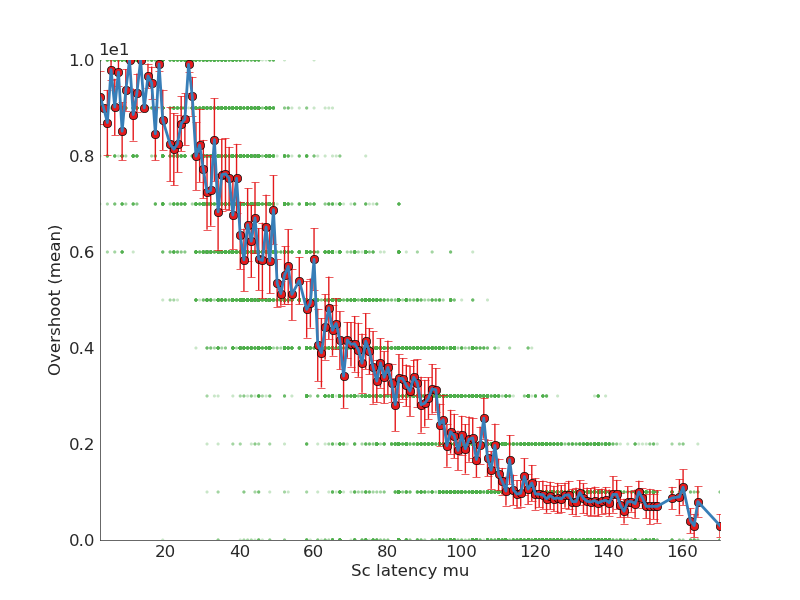
\includegraphics[width=0.5\textwidth]{101_pars_vs_fits/d10/sc_latency_mu__vs__overshoot(mean)_scatter.png}}
	\subcaptionbox{Correlation between \sclatencymu and \roundstable\label{fig:d10_parvfit_sclatencymu_b}}
	[0.49\linewidth]{\includegraphics[width=0.5\textwidth]{101_pars_vs_fits/d10/sc_latency_mu__vs__round_stable(mean)_scatter.png}}
	\subcaptionbox{Correlation between \sclatencymu and \stdev\label{fig:d10_parvfit_sclatencymu_c}}
	[0.49\linewidth]{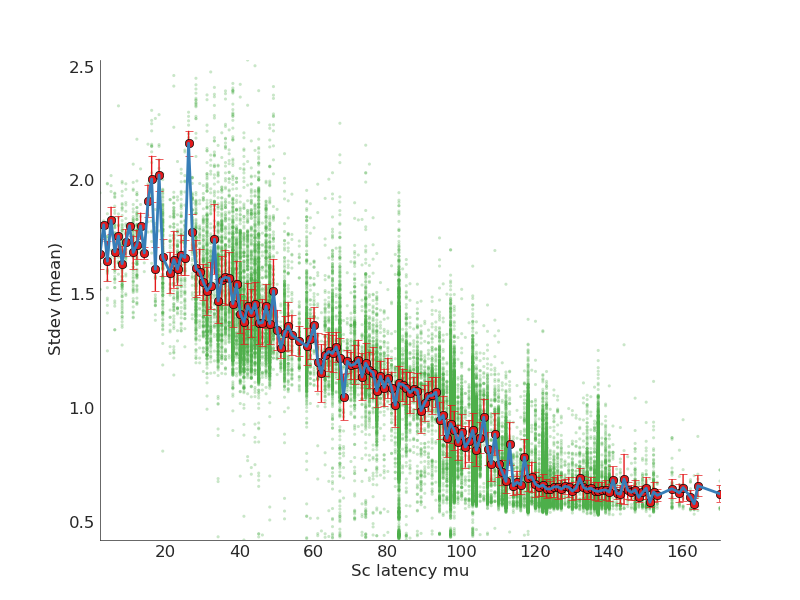
\includegraphics[width=0.5\textwidth]{101_pars_vs_fits/d10/sc_latency_mu__vs__stdev(mean)_scatter.png}}
	\subcaptionbox{Correlation between \sclatencymu and \timetoreachnewfundamental\label{fig:d10_parvfit_sclatencymu_d}}
	[0.49\linewidth]{\includegraphics[width=0.5\textwidth]{101_pars_vs_fits/d10/sc_latency_mu__vs__time_to_reach_new_fundamental(mean)_scatter.png}}
	\caption{Correlation between \sclatencymu and the four fitness measures in experiment \dten}
	\label{fig:d10_parvfit_sclatencymu}
\end{figure}
The list below briefly summarizes the results shown by figure \ref{fig:d10_parvfit_sclatencymu}.

Figure \ref{fig:d10_parvfit_sclatencymu_a} shows that \sclatencymu is negatively correlated with \overshoot, such that markets with faster chartists are more likely to have a larger overshoot. Since all simulations with $\overshoot>10$ were considered outliers and therefore removed, the vertical axis is limited to $\overshoot = 10$. Next, figure \ref{fig:d10_parvfit_sclatencymu}  shows that \sclatencymu is negatively correlated with \stdev, such that markets with faster chartists are more likely to have flickering trade prices. 

As for the market responsiveness, it is seen that \sclatencymu is positively correlated with \timetoreachnewfundamental, such that markets with faster agents is more likely to have a shorter response time to the market. Figure \ref{fig:d10_parvfit_sclatencymu_d} confirms that markets with fast chartists did actually manage to reach the new fundamental price faster than those markets having slow chartists. The average response time of markets in which the chartists had a latency of less than 30 rounds was around 18000 rounds, whereas it was around 25000 rounds with chartists with more than 100 rounds of latency. The market response time is most sensitive in the range $20< \sclatencymu<60$, and does not change much for larger latencies. 

The plots of \overshoot, \stdev and \timetoreachnewfundamental show that predicting the three fitness measures in markets with slow chartists would be more accurate than for markets with fast chartists, as the correlation of \overshoot, \stdev and \timetoreachnewfundamental with \sclatencymu is stronger for larger values of \sclatencymu. 

Figure \ref{fig:d10_parvfit_sclatencymu_b} shows that \sclatencymu is positively correlated with \roundstable, but also that the relationship between \sclatencymu and \roundstable seems highly non-linear. The figure illustrates the binary nature of the stability criteria, that is, that a simulation is either stable or not stable. This causes \roundstable to have a high conditional variance of \roundstable given \sclatencymu in the region $50 < \sclatencymu < 120$, meaning that that prediction of \roundstable from \sclatencymu in this region would not be very accurate. What this means is that the stability of a simulation is highly dependent on factors other than \sclatencymu, when the parameter is within 50 to 120 rounds. When the chartists are faster than 50 rounds, the market is almost always unstable, and when the chartists are slower than 120 rounds the market is almost always stable. 

\subsubsection*{Number of market makers}
\begin{figure}
	%issue 15
	\centering
	\subcaptionbox{Correlation between \ssmmnAgents{} and \overshoot\label{fig:d10_parvfit_ssmmnAgents_a}}
	[0.49\linewidth]{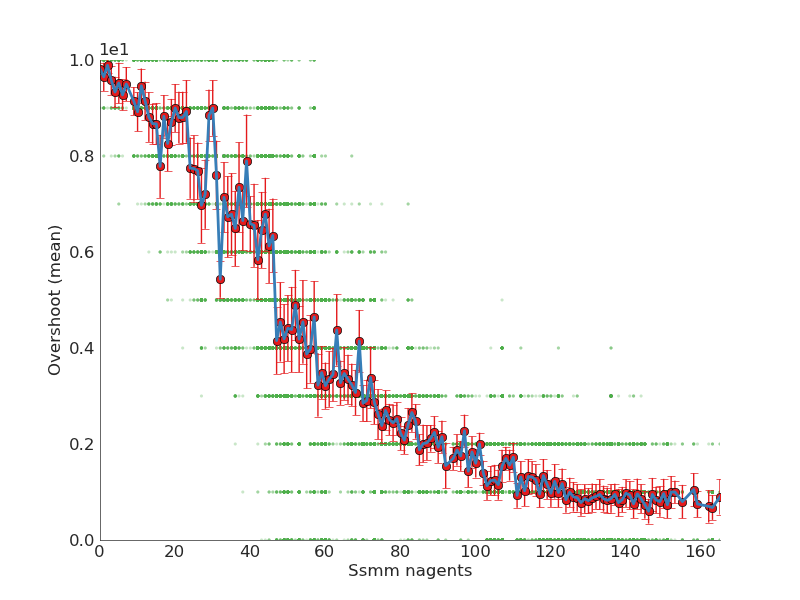
\includegraphics[width=0.5\textwidth]{101_pars_vs_fits/d10/ssmm_nAgents__vs__overshoot(mean)_scatter.png}}
	\subcaptionbox{Correlation between \ssmmnAgents{} and \roundstable\label{fig:d10_parvfit_ssmmnAgents_b}}
	[0.49\linewidth]{\includegraphics[width=0.5\textwidth]{101_pars_vs_fits/d10/ssmm_nAgents__vs__round_stable(mean)_scatter.png}}
	\subcaptionbox{Correlation between \ssmmnAgents{} and \stdev\label{fig:d10_parvfit_ssmmnAgents_c}}
	[0.49\linewidth]{\includegraphics[width=0.5\textwidth]{101_pars_vs_fits/d10/ssmm_nAgents__vs__stdev(mean)_scatter.png}}
	\subcaptionbox{Correlation between \ssmmnAgents{} and \timetoreachnewfundamental\label{fig:d10_parvfit_ssmmnAgents_d}}
	[0.49\linewidth]{\includegraphics[width=0.5\textwidth]{101_pars_vs_fits/d10/ssmm_nAgents__vs__time_to_reach_new_fundamental(mean)_scatter.png}}
	\caption{Correlation between \ssmmnAgents and the four fitness measures in experiment \dten}
	\label{fig:d10_parvfit_ssmmnAgents}
\end{figure}
Figure, \ref{fig:d10_parvfit_ssmmlatencymu}, showing the how the number of market makers correlates with the model fitness, is quite similar to figure \ref{fig:d10_parvfit_sclatencymu}. A large number of market makers reduces the overshoot, whereas the virtually always have an overshoot when there are little or no market makers. The same is true for the flickering of the trade prices: few market makers always means flickering prices. A higher number of market makers makes the market less responsive, while fewer market makers makes the market more responsive. Finally, the number of market makers also influences how quickly the market settles within the stability margin, as markets with more market makers become stable faster than markets with few agents. However, figure \ref{fig:d10_parvfit_ssmmlatencymu_b} shows that it sometimes happens that a market with few market makers becomes stable quickly.

\begin{enumerate}
\item When the market has fast chartists, it needs more market makers to keep the market stable, but these may be slow.
\item When the market has fast chartists, the market first of all needs fast market makers to be stable.
\item A market with few market makers can be stable if the market makers are fast, or if the chartists are slow.
\end{enumerate}

\subsubsection*{Market maker latency}
\begin{figure}
	%issue 15
	\centering
	\subcaptionbox{Correlation between \ssmmlatencymu and \overshoot\label{fig:d10_parvfit_ssmmlatencymu_a}}
	[0.49\linewidth]{\includegraphics[width=0.5\textwidth]{101_pars_vs_fits/d10/ssmm_latency_mu__vs__overshoot(mean)_scatter.png}}
	\subcaptionbox{Correlation between \ssmmlatencymu and \roundstable\label{fig:d10_parvfit_ssmmlatencymu_b}}
	[0.49\linewidth]{\includegraphics[width=0.5\textwidth]{101_pars_vs_fits/d10/ssmm_latency_mu__vs__round_stable(mean)_scatter.png}}
	\subcaptionbox{Correlation between \ssmmlatencymu and \stdev\label{fig:d10_parvfit_ssmmlatencymu_c}}
	[0.49\linewidth]{\includegraphics[width=0.5\textwidth]{101_pars_vs_fits/d10/ssmm_latency_mu__vs__stdev(mean)_scatter.png}}
	\subcaptionbox{Correlation between \ssmmlatencymu and \timetoreachnewfundamental\label{fig:d10_parvfit_ssmmlatencymu_d}}
	[0.49\linewidth]{\includegraphics[width=0.5\textwidth]{101_pars_vs_fits/d10/ssmm_latency_mu__vs__time_to_reach_new_fundamental(mean)_scatter.png}}
	\caption{Correlation between \sclatencymu and the four fitness measures in experiment \dten}
	\label{fig:d10_parvfit_ssmmlatencymu}
\end{figure}

The market almost never has any overshoot, irregardless 

The tricky thing about this


\begin{enumerate}
\setcounter{enumi}{1}
\item The time it takes for the market to become stable depends on the number of market makers and on the latency of the market makers. More and slower market makers seems to make the market settle within the stability margin faster.
\end{enumerate}



\subsubsection{Number of chartists}
\begin{figure}
	%issue 15
	\centering
	\subcaptionbox{Correlation between \scnAgents and \overshoot\label{fig:d10_parvfit_scnagents_a}}
	[0.49\linewidth]{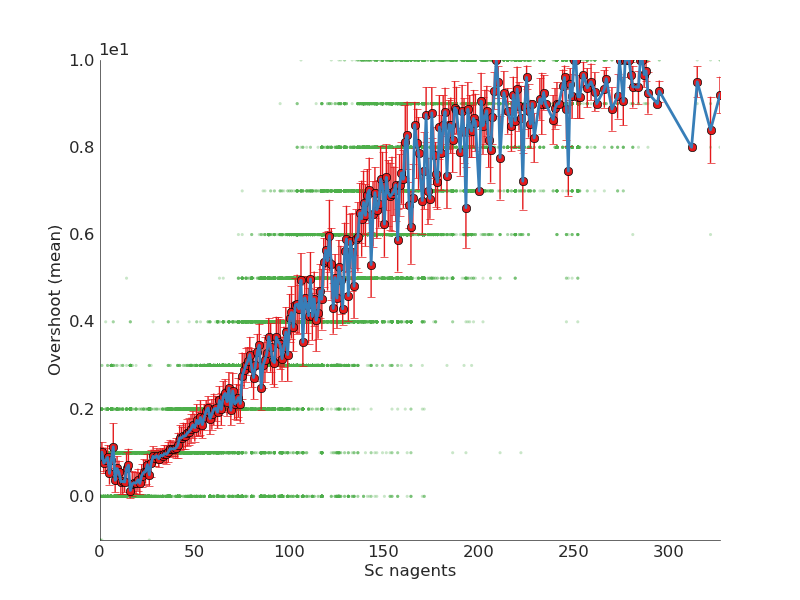
\includegraphics[width=0.5\textwidth]{101_pars_vs_fits/d11/sc_nAgents__vs__overshoot(mean)_scatter.png}}
	\subcaptionbox{Correlation between \scnAgents and \roundstable\label{fig:d10_parvfit_scnagents_b}}
	[0.49\linewidth]{\includegraphics[width=0.5\textwidth]{101_pars_vs_fits/d11/sc_nAgents__vs__round_stable(mean)_scatter.png}}
	\subcaptionbox{Correlation between \scnAgents and \stdev\label{fig:d10_parvfit_scnagents_c}}
	[0.49\linewidth]{\includegraphics[width=0.5\textwidth]{101_pars_vs_fits/d11/sc_nAgents__vs__stdev(mean)_scatter.png}}
	\subcaptionbox{Correlation between \scnAgents and \timetoreachnewfundamental\label{fig:d10_parvfit_scnagents_d}}
	[0.49\linewidth]{\includegraphics[width=0.5\textwidth]{101_pars_vs_fits/d11/sc_nAgents__vs__time_to_reach_new_fundamental(mean)_scatter.png}}
	\caption{Correlation between \scnAgents and the four fitness measures in experiment \dten}
	\label{fig:d10_parvfit_scnagents}
\end{figure}



\subsubsection{Chartist- to market maker ratio}




\begin{enumerate}
\setcounter{enumi}{2}
\item The overshoot of the market seems to be influenced by all three factors, as did the fluctuations of the traded prices.
\end{enumerate}
As figure \ref{fig:d10_parvfit_sclatencymu_a} shows, the overshoot seems to be highly correlated with the latency of the chartists.


\ref{fig:d10_parvfit_sclatencymu_c} and \ref{fig:d10_parvfit_ssmmnAgents_a} \ref{fig:d10_parvfit_ssmmnAgents_c}

and somewhat true for

\ref{fig:d10_parvfit_ssmmnAgents_a} and \ref{fig:d10_parvfit_ssmmnAgents_c}



\begin{enumerate}
\setcounter{enumi}{3}
\item The market was more stable but reacted slowly when the chartists were slower than the market makers.
\end{enumerate}






\subsection{Clustering}
In this section, the focus is shifted from looking at population wide statistics to analysis sub-groups within each population. Whereas the previous sections showed that there do indeed exist statistical relationships between the latency of the agents and the behavior of the model, each discovered correlation was calculated over the entire population. 

For instance, even though prediction of, say a negative correlation between \timetoreachnewfundamental was \sclatencymu was found, there might be configurations of the model in which faster chartists were actually beneficial to the market. In order to investigate this, a Gaussian mixture model (GMM) was used to find clusters in the fitness space. All four fitness measures were used for the clustering. After discarding simulations with undefined fitness values and removing outliers, the data set contained 80813 data points. The large number of data points and the low number of dimensions made it possible to allow a each Gaussian component to have a full covariance matrix, giving the model a high level of flexibility. Figure \ref{fig:d10_scatter_clusters} shows scatter plots of the data after it has been grouped. Tables \ref{table:fit_gmm_all_mean} and \ref{table:fit_gmm_all_std} respectively show the mean and standard deviation calculated over each cluster. The tables are sorted by the average value of \overshoot.



\begin{figure}
	%issue 15
	\centering
	\subcaptionbox{}[0.49\linewidth]{\includegraphics[width=0.5\textwidth]{manually_selected/108_cluster_after_removing_outliers/d10/12_gmm_all_fit_0.png}}
	\subcaptionbox{}[0.49\linewidth]{\includegraphics[width=0.5\textwidth]{manually_selected/108_cluster_after_removing_outliers/d10/12_gmm_all_fit_1.png}}
	\subcaptionbox{}[0.49\linewidth]{\includegraphics[width=0.5\textwidth]{manually_selected/108_cluster_after_removing_outliers/d10/12_gmm_all_fit_2.png}}
	\caption{Scatter plots in fitness space showing the grouping of data points when using a GMM with 12 clusters.}
	\label{fig:d10_scatter_clusters}
\end{figure}


$\Varcluster{\roundstable}{8}$ and $\Varcluster{\roundstable}{11}$ and $\Varcluster{\roundstable}{5}$ are large. The points in this cluster have parameters which 



\subsubsection*{Chartist latency and market response time}
As was noted earlier, the evolution of \sclatencymu and \timetoreachnewfundamental indicates that slow chartists made the market slow, and fast chartists made the market fast. C1 is the cluster with the $\Ecluster{\timetoreachnewfundamental}{1}$

\begin{table}
 \centering
 \begin{tabular}{l|rrrr|rrrrrr}
\toprule
{} &  \overshoot &  \roundstable &  \stdev &  \timetoreachnewfundamental &  \sclatencymu &  \sclatencys &  \ssmmlatencymu &  \ssmmlatencys &  \ssmmnAgents &  \Count \\
\midrule
C1  &         0.0 &       16301.2 &     0.6 &                     19217.4 &         127.2 &          6.2 &            78.4 &            5.2 &         132.2 &  7803 \\
C7  &         0.3 &       24383.1 &     0.7 &                     32005.5 &          87.0 &          9.5 &            25.8 &           10.5 &          66.7 &  1012 \\
C10 &         1.0 &       15832.8 &     0.7 &                     18602.8 &         121.9 &          6.5 &            76.3 &            6.0 &         126.3 & 25245 \\
C8  &         2.0 &       81599.7 &     0.9 &                     16333.6 &         101.8 &          8.7 &            56.4 &            9.2 &          91.3 &  7442 \\
C11 &         2.0 &       30515.0 &     0.7 &                     17822.9 &         114.2 &          7.3 &            71.7 &            7.0 &         117.5 &  5056 \\
C0  &         3.0 &       89015.0 &     1.1 &                     14687.5 &          89.0 &          9.2 &            39.5 &           10.0 &          66.8 &  9201 \\
C5  &         3.0 &       51306.4 &     0.9 &                     16508.7 &         102.2 &          9.0 &            59.2 &            8.8 &          96.0 &   356 \\
C6  &         3.0 &       83914.2 &     1.1 &                     16820.9 &          92.3 &          9.2 &            40.6 &           10.0 &          72.4 &  1598 \\
C9  &         4.0 &       89496.0 &     1.2 &                     14459.8 &          77.7 &          9.6 &            29.9 &           10.4 &          56.7 &  7278 \\
C4  &         5.0 &       89896.6 &     1.4 &                     22034.2 &          62.4 &          9.4 &            21.5 &           10.3 &          51.6 &  5331 \\
C3  &         6.7 &       86440.9 &     1.8 &                     18692.7 &          54.9 &          9.2 &            26.2 &           10.5 &          38.0 &   390 \\
C2  &         7.9 &       89996.1 &     1.6 &                     11574.7 &          36.4 &          9.2 &            26.4 &            9.6 &          36.4 &  10101 \\
Outliers  &        11.5 &       89998.8 &     2.2 &                      8835.1 &          17.8 &          9.3 &            24.3 &            8.5 &          19.4 &   740 \\
\bottomrule
\end{tabular}
 \label{table:fit_gmm_all_mean}
 \caption{Mean for each fitness-cluster.}
 \end{table}
 
 C2 contains the fastest simulations, which take an average of $11.5\times 10^3$ rounds to reach the new fundamental. This group is also the one with the largest overshoot. 

\begin{table}
 \centering
 \begin{tabular}{l|rrrr|rrrrrr}
\toprule
{} &  \overshoot &  \roundstable &  \stdev &  \timetoreachnewfundamental &  \sclatencymu &  \sclatencys &  \ssmmlatencymu &  \ssmmlatencys &  \ssmmnAgents &  \Count \\
\midrule
C1  &         0.0 &        2142.8 &     0.0 &                      2220.9 &          10.9 &          4.7 &             7.1 &            3.3 &          11.3 &  7803 \\
C7  &         0.5 &        4827.7 &     0.2 &                      7424.7 &          18.4 &          3.8 &            18.7 &            5.4 &          23.2 &  1012 \\
C10 &         0.0 &        2150.8 &     0.1 &                      2261.1 &          12.7 &          4.7 &             9.3 &            4.1 &          14.7 & 25245 \\
C8  &         0.0 &       10563.6 &     0.1 &                      1926.7 &          10.3 &          4.0 &            12.2 &            5.3 &          20.0 &  7442 \\
C11 &         0.0 &        6952.5 &     0.1 &                      2276.1 &          13.8 &          4.7 &            11.6 &            4.7 &          18.3 &  5056 \\
C0  &         0.0 &        1380.7 &     0.1 &                      1479.2 &           9.7 &          3.4 &            14.7 &            5.0 &          12.7 &  9201 \\
C5  &         0.0 &       17151.2 &     0.1 &                      2087.1 &          11.2 &          4.2 &            12.5 &            5.2 &          21.4 &   356 \\
C6  &         0.0 &        3961.3 &     0.1 &                      2646.9 &          10.3 &          3.5 &            16.9 &            5.2 &          16.0 &  1598 \\
C9  &         0.0 &        1048.5 &     0.1 &                      2368.7 &          13.0 &          3.4 &            12.7 &            4.9 &           9.4 &  7278 \\
C4  &         1.4 &         423.6 &     0.2 &                      4246.5 &          21.3 &          4.3 &            11.6 &            5.3 &          10.4 &  5331 \\
C2  &         1.6 &         211.8 &     0.2 &                      1943.0 &          16.0 &          5.2 &            11.7 &            5.5 &          13.7 & 10101 \\
C3  &         2.9 &        7387.0 &     0.4 &                     11884.0 &          26.0 &          4.5 &            15.0 &            5.5 &          30.6 &   390 \\
Outliers  &         0.8 &           0.6 &     0.3 &                      2691.9 &          11.3 &          6.1 &            13.4 &            5.7 &          14.2 &   740 \\
\bottomrule
\end{tabular}
 \label{table:fit_gmm_all_std}
 \caption{Standard deviation for each fitness-cluster.}
 \end{table}


The point of the clustering is not that all groups should have distinctly different parameter statistics. 
 
 \begin{figure}
 \centering
 \begin{minipage}[t]{.5\linewidth}
 \vspace{25pt}
 \centering
 \begin{tabular}{lrrrrrr}
\toprule
{} &  \sclatencymu &  \sclatencys &  \ssmmlatencymu &  \ssmmlatencys &  \ssmmnAgents &  $\gamma$ \\
\midrule
0 &          0.53 &        -0.24 &            0.54 &          -0.24 &          0.56 &    0.57 \\
1 &          -0.0 &         0.74 &           -0.01 &          -0.67 &          0.03 &    0.18 \\
2 &          0.23 &         0.63 &            0.16 &            0.7 &          0.19 &    0.17 \\
\bottomrule
\end{tabular}
\end{minipage}%
\begin{minipage}[t]{.5\linewidth}
\vspace{0pt}
\centering
\includegraphics[width=0.75\linewidth]{manually_selected/108_cluster_after_removing_outliers/d10/clustering_d10_allclusters.png}
\end{minipage}
\label{table:clustering_d10_allclusters}
\caption{XXX}
\end{figure}
%Component 0:
%\[\sclatencymu=0.532, \sclatencys=-0.235, \ssmmlatencymu=0.544, \ssmmlatencys=-0.239, \ssmmnAgents=0.555\]
%Component 1:
%\[\sclatencymu=0.532, \sclatencys=-0.235, \ssmmlatencymu=0.544, \ssmmlatencys=-0.239, \ssmmnAgents=0.555\]
%Component 2:
%\[\sclatencymu=0.532, \sclatencys=-0.235, \ssmmlatencymu=0.544, \ssmmlatencys=-0.239, \ssmmnAgents=0.555\]



\begin{comment}
\section{D11}\label{section:experiment_9}

\begin{figure}
	%issue 15
	\centering
	\subcaptionbox{Evolution of \ssmmlatencymu{} and \sclatencymu}
	[0.49\linewidth]{\includegraphics[width=0.5\textwidth]{82_generation_plots/d11/latpars_mu.png}}
	\subcaptionbox{Evolution of \ssmmlatencys{} and \sclatencys}
	[0.49\linewidth]{\includegraphics[width=0.5\textwidth]{82_generation_plots/d11/latpars_s.png}}
	\subcaptionbox{Evolution of \scnAgents}
	[0.49\linewidth]{\includegraphics[width=0.5\textwidth]{82_generation_plots/d11/nAgents.png}}
	\caption{Evolution of the model parameters in experiment \deleven}
	\label{fig:d11_evolution_parameters}
\end{figure}

\begin{figure}
	%issue 15
	\centering
	\subcaptionbox{Evolution of \roundstable}
	[0.49\linewidth]{\includegraphics[width=0.5\textwidth]{82_generation_plots/d11/round_stable.png}}
	\subcaptionbox{Evolution of \timetoreachnewfundamental}
	[0.49\linewidth]{\includegraphics[width=0.5\textwidth]{82_generation_plots/d11/time_to_reach_new_fundamental.png}}
	\subcaptionbox{Evolution of \stdev}
	[0.49\linewidth]{\includegraphics[width=0.5\textwidth]{82_generation_plots/d11/stdev.png}}
	\subcaptionbox{Evolution of \overshoot}
	[0.49\linewidth]{\includegraphics[width=0.5\textwidth]{82_generation_plots/d11/overshoot.png}}
	\caption{Evolution of the four fitness measures in experiment \deleven}
	\label{fig:d11_evolution_fitness}
\end{figure}

\begin{figure}
	%issue 15
	\centering
	\subcaptionbox{Correlation between \sclatencymu{} and \overshoot}
	[0.49\linewidth]{\includegraphics[width=0.5\textwidth]{101_pars_vs_fits/d11/sc_latency_mu__vs__overshoot(mean)_scatter.png}}
	\subcaptionbox{Correlation between \sclatencymu{} and \roundstable}
	[0.49\linewidth]{\includegraphics[width=0.5\textwidth]{101_pars_vs_fits/d11/sc_latency_mu__vs__round_stable(mean)_scatter.png}}
	\subcaptionbox{Correlation between \sclatencymu{} and \stdev}
	[0.49\linewidth]{\includegraphics[width=0.5\textwidth]{101_pars_vs_fits/d11/sc_latency_mu__vs__stdev(mean)_scatter.png}}
	\subcaptionbox{Correlation between \sclatencymu{} and \timetoreachnewfundamental}
	[0.49\linewidth]{\includegraphics[width=0.5\textwidth]{101_pars_vs_fits/d11/sc_latency_mu__vs__time_to_reach_new_fundamental(mean)_scatter.png}}
	
	\caption{Correlation between \sclatencymu and the four fitness measures in experiment \deleven}
	\label{fig:d11_parvfit_sclatencymu}
\end{figure}

\begin{figure}
	%issue 15
	\centering
	\subcaptionbox{Correlation between \ssmmlatencymu{} and \overshoot}
	[0.49\linewidth]{\includegraphics[width=0.5\textwidth]{101_pars_vs_fits/d11/ssmm_latency_mu__vs__overshoot(mean)_scatter.png}}
	\subcaptionbox{Correlation between \ssmmlatencymu{} and \roundstable}
	[0.49\linewidth]{\includegraphics[width=0.5\textwidth]{101_pars_vs_fits/d11/ssmm_latency_mu__vs__round_stable(mean)_scatter.png}}
	\subcaptionbox{Correlation between \ssmmlatencymu{} and \stdev}
	[0.49\linewidth]{\includegraphics[width=0.5\textwidth]{101_pars_vs_fits/d11/ssmm_latency_mu__vs__stdev(mean)_scatter.png}}
	\subcaptionbox{Correlation between \ssmmlatencymu{} and \timetoreachnewfundamental}
	[0.49\linewidth]{\includegraphics[width=0.5\textwidth]{101_pars_vs_fits/d11/ssmm_latency_mu__vs__time_to_reach_new_fundamental(mean)_scatter.png}}
	
	\caption{Correlation between \sclatencymu{} and the four fitness measures in experiment \deleven}
	\label{fig:d11_parvfit_ssmmlatencymu}
\end{figure}


\begin{figure}
	%issue 15
	\centering
	\subcaptionbox{Correlation between \scnAgents{} and \overshoot}
	[0.49\linewidth]{\includegraphics[width=0.5\textwidth]{101_pars_vs_fits/d11/sc_nAgents__vs__overshoot(mean)_scatter.png}}
	\subcaptionbox{Correlation between \scnAgents{} and \roundstable}
	[0.49\linewidth]{\includegraphics[width=0.5\textwidth]{101_pars_vs_fits/d11/sc_nAgents__vs__round_stable(mean)_scatter.png}}
	\subcaptionbox{Correlation between \scnAgents{} and \stdev}
	[0.49\linewidth]{\includegraphics[width=0.5\textwidth]{101_pars_vs_fits/d11/sc_nAgents__vs__stdev(mean)_scatter.png}}
	\subcaptionbox{Correlation between \scnAgents{} and \timetoreachnewfundamental}
	[0.49\linewidth]{\includegraphics[width=0.5\textwidth]{101_pars_vs_fits/d11/sc_nAgents__vs__time_to_reach_new_fundamental(mean)_scatter.png}}
	
	\caption{Correlation between \ssmmnAgents{} and the four fitness measures in experiment \deleven}
	\label{fig:d11_parvfit_scAgents}
\end{figure}
\end{comment}


\section{Hall of fame}\label{section:hall_of_fame}
